
\documentclass[12pt]{amsart}
\usepackage{geometry} % see geometry.pdf on how to lay out the page. There's lots.
\geometry{a4paper} % or letter or a5paper or ... etc
\usepackage{graphicx}
% \geometry{landscape} % rotated page geometry

% See the ``Article customise'' template for come common customisations

\title{ Space is the Place: How Dispersal and Competition Shape Genetic Variation in Continuous Space }
\author{C. J. Battey, Peter Ralph, Andrew Kern}
\date{November 2018} % delete this line to display the current date

%%% BEGIN DOCUMENT
\begin{document}

\maketitle
\tableofcontents

\section{Abstract}

\section{Introduction}
Random mating is a core assumption of many population genetic models, but likely occurs in few real populations. Instead most organisms mate with nearby individuals and disperse across only a small part of the full range of a species. This process creates the pattern known as isolation by distance (IBD; Wright 1942) -- a positive correlation between genetic and geographic distances among individuals. Though this pattern is both expected from first principles and widely observed in natural populations (Aguillon et al. 2017, Pinto et al. 2013, Battey et al. 2018), existing population genetic models either exclude it entirely (by assuming random mating) or take the heuristic approach of binning the landscape into discrete blocks of randomly mating populations that exchange migrants each generation. 

Efforts to model genomes evolving in continuous space have a long history but have been limited by computational inefficiency and a lack of analytic tractability. Both Wright (1942) and Malecót (196X) developed analytic expectations for genetic variation of populations in continuous space, but these models fail to capture the spatial dynamics of real populations (Felsenstein XXXX). Specifically, the externally fixed population sizes used in Wright's and Malecót's models creates a form of global population regulation in which the fitness of each individual depends on the fitness of every other individual in the population despite a lack of interaction among distant individuals. Over time this causes populations to become increasingly clumped until all individuals occur in a single contiguous area occupying a fraction of the available range -- what Felsenstein 197X described as "the pain in the torus". 

In reality global population size is an emergent property of individual fitness, which in turn is regulated by competition among interacting individuals at the local scale. 

\section{Methods}
\subsection{ A Forward-Time Model of Evolution in Continuous Space }

\subsubsection{ Mating and Dispersal } 

\subsubsection{ Competition } 

\subsubsection{ Boundary Conditions (Refrain from the Torus?) } 

\subsubsection{ Tree Sequence Recording } 

\subsection{ Summary Statistics } 

\subsection{ Demographic Modeling }

\subsection{ Association Tests } 

\subsection{ Machine Learning }


\section{Results}

\subsection{ Summary Statistics }

\subsection{ Impacts on Demographic Inference and GWAS }

\subsection{ Estimating Model Parameters with Machine Learning }


\section{ Discussion } 

\section{Figures}


\begin{figure}[h]
	\centerline{
	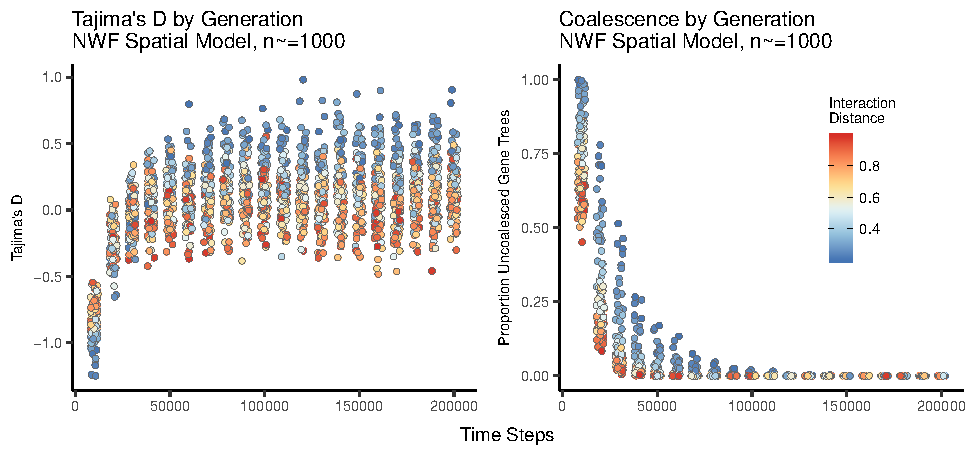
\includegraphics{../figures/10kouts_coalescence_by_generation}
	}
\end{figure}


\begin{figure}[h]
	\centerline{
	\includegraphics{../figures/sumstat_by_neighbors_spat_v_rm.pdf}
	}
\end{figure}

\begin{figure}[h]
	\centerline{
	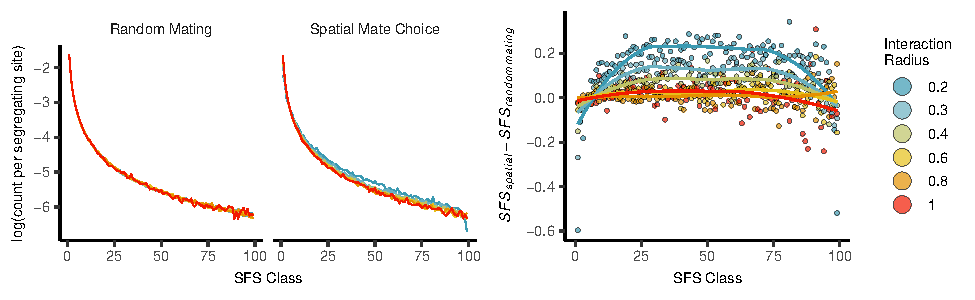
\includegraphics{../figures/sfs_spatial_v_rm.pdf}
	}
\end{figure}


\end{document}